\documentclass{article}

\usepackage{../preamble}
\standalonetrue

\pagestyle{fancy}
\fancyhf{}
\rhead{Section \thesection}
\lhead{PHYS 304 Lecture 12}
\rfoot{Page \thepage}


\title{PHYS 304 Lecture 12}
\author{Ashtan Mistal}
\date{!!!}

\begin{document}

\ifstandalone
\maketitle
\fi

\graphicspath{{./Lecture12/}}


\section{Recap}


\begin{itemize}
    \item In 2D Real space, $|\vec{r}\rangle \cong\left[\begin{array}{l}x \\ y\end{array}\right] ;\langle\vec{r}| \cong\left[\begin{array}{ll}x & y\end{array}\right]=\left[\begin{array}{l}x \\ y\end{array}\right]^{\top}$
    
    \item $\langle\gamma \| \gamma\rangle \equiv\left\langle\gamma \mid \gamma^{\prime}\right\rangle=x x^{\prime}+y y^{\prime} \in \mathbb{R}$
    
    \item $\left\{\left|\alpha_{1}\right\rangle,\left|\alpha_{2}\right\rangle\right\} \Rightarrow$ Orthonormal basis.
    \begin{enumerate}
        \item Orthonormality $\Rightarrow\left\langle\alpha_{i} \mid \alpha_{j}\right\rangle=\delta_{i j}$
        
        \item Completeness $\Rightarrow \sum_{i=1}^{2}\left|\alpha_{i}\right\rangle\left\langle\alpha_{i}\right|=\mathbb{I} \quad \begin{aligned}&\text { Resolution of the } \\&\text { identity operator. }\end{aligned}$
        
        \item $P_i$ are the projectors
    \end{enumerate}
    
    \item The rotation operator:

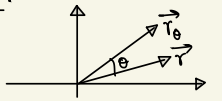
\includegraphics[width = 0.3 \textwidth]{Lecture12/1.png}

$$R_{\theta}|\vec{r}\rangle =\left|\vec{\gamma}_{\theta}\right\rangle$$

$$=\sum_{j=1}^{2} R_{\theta}\left|\alpha_{j}\right\rangle\left\langle\alpha_{j} \mid \vec{r}\right\rangle$$

$$\Rightarrow\left\langle\alpha_{i} \mid \vec{r}_{\theta}\right\rangle =\sum_{j=1}^{2} \underbrace{ \left\langle\alpha_{i}\left|R_{\theta}\right| \alpha_{j}\right\rangle}_{\text{Matrix elements of } R_{\theta} \text{ in } \alpha_{i}, \alpha_{j} \text{ basis!}} \left\langle\alpha_{j} \mid \vec{r}\right\rangle$$

\item $\left(\hat{R}_{\theta}\right)_{i j}=\left[\begin{array}{cc}
\cos \theta & -\sin \theta \\
\sin \theta & \cos \theta
\end{array}\right]$

\end{itemize}

\section{Complex Vector Spaces}

Although the space $\mathbb{R}^{2}$ is most intuitive to us, QM has complex numbers in built. (See TDSE!!)

\begin{itemize}
    \item A Complex inner pdt has properties :
\begin{itemize}
\item (i) $\langle u \mid v\rangle=\langle v \mid u\rangle^{*}$.
    \item $\langle u \mid u\rangle \geqslant 0$ equality satistifed iff $u=0$
    \item Sesquilinear:
    \begin{itemize}
        \item $\left\langle u \mid c_{1} v_{1}+c_{2} v_{2}\right\rangle=c_{1}\left\langle u \mid v_{1}\right\rangle+c_{2}\left\langle u \mid v_{2}\right\rangle$
        \item  $\left\langle c_{1} u_{1}+c_{2} u_{2} \mid \nabla\right\rangle=c_{1}^{*}\left\langle u_{1} \mid v\right\rangle+c_{2}^{*}\left\langle u_{2} \mid v\right\rangle$
    \end{itemize}
\end{itemize} 


\item Concrete examples: 

\begin{itemize}
    \item $a=\left(\begin{array}{l}a_{1} \\ a_{2}\end{array}\right) ; b=\left(\begin{array}{l}b_{1} \\ b_{2}\end{array}\right)$ where $x_{1}, y_{i} \in \psi$
    $$
\langle a \mid b\rangle \equiv a_{1}^{*} b_{1}+a_{2}^{*} b_{2} \in \phi
$$

\item  Consider two Complex valued functions $ f(x), g(x) \in \&$ in $L^{2}(\mathbb{R})$
$\langle f \mid g\rangle=\int_{-\infty}^{\infty} d x f^{*}(x) g(x)$
\end{itemize} 


Note that if $\underset{\text { "ket" }}{|a\rangle}=\left(\begin{array}{c}a_{1} \\ a_{2} \\ \vdots \\ a_{N}\end{array}\right) \leftrightarrow\left\langle_{n} b_{a_{1}^{\prime \prime}}=\left(a_{1}^{*} a_{2}^{*} \ldots \ldots a_{N}^{*}\right)\right.$

\item Question: if $|v\rangle=\alpha_{1}\left|v_{1}\right\rangle+\alpha_{2}\left|v_{2}\right\rangle$ then what is $\langle v| ? =\alpha_{1}^{*}\left\langle v_{1}\right|+\alpha_{2}^{*}\left\langle v_{2}\right|$

$\Rightarrow \text { Abstractly: }\underbrace{\langle v \mid u\rangle}_{\text { property of inner pdt}} =\langle u \mid v\rangle^{*}=\left\langle u \mid \alpha_{1} v_{1}\right\rangle^{*}+\left\langle u \mid \alpha_{2} v_{2}\right\rangle^{*}=\alpha_{1}^{*}\left\langle v_{1} \mid u\right\rangle+\alpha_{2}^* \left\langle v_{2} \mid u\right\rangle = \left( \alpha_i^* \bra{v_1} + \alpha_2^* \bra{v_2} \right) \ket{u}$

Where the inner product property is applied once in each step (of the equals sign). 

Here, if you have an ONB $\{|i\rangle\}$, any vector $V$ can be expanded as:
$$
|v\rangle=\sum_{i}|i\rangle\langle i \mid v\rangle=\sum_{i} c_{i}|i\rangle \text { where } G \equiv\langle i \mid v\rangle
$$

\end{itemize}


\subsection{Operators and Matrix elements:}
\begin{itemize}
    \item Operators are objects that eat a vector and spit out some different vector.
$$
\begin{aligned}
0: V & \rightarrow V \\
|V\rangle & \mapsto 0|V\rangle
\end{aligned}
$$
\item $O$ is naturally written as $0=|a\rangle\langle v|$
\item  $0=\sum_{i, j} \mid \underbrace{\langle i\rangle \mid j}_{0_{i j} \rightarrow \text { matrix elements. }}$
\item Note this notation is self-correcting: 

\begin{itemize}
    \item Matrix multiplication: $\langle A B)_{i j}=\langle i|A B| j\rangle$
$$
\begin{aligned}
&=\sum_{k}\langle i|A| k\rangle\langle k|B| j\rangle \\
&=\sum_{k} A_{i k} B_{k j}
\end{aligned}
$$
\end{itemize} 
\end{itemize}


\section{Adjoint of a linear operator}

$$\underbrace{\braket{u | Ov}}_{\braket{u | O | v}} \equiv \braket{O^+ u | v} \forall u,v \in \mathbb{V}$$

Conjugate: $\braket{O v | u} = \braket{v | O^+ | u} \Rightarrow \bra{v } O^+ = \bra{Ov}$

The bra associated with $O \ket{v}$ is $\bra{v} O^+$

Now note $\braket{u|O|v}^* = \braket{v|O^+|u}$; if we choose $u,v$ as ONB \footnote{ONB = orthonormal basis. } vectors:

$$\braket{i | O^+|u} = \braket{j|O|i}^*$$

$$\Rightarrow (O^+)_{ij} = \underbrace{O_{ji}^*}_{\text{Explicit matrix elements!}}$$

Exercise: If $O = \ket{a} \bra{b}$, write $O^+ = ? \rightarrow O^+ = \ket{b} \bra{a}$

$$O \ket{v} = \ket{a} \braket{b|v} = \braket{b|v} \ket{a} \longrightarrow \bra{v} O^+ = \bra{v} \ket{b} \bra{a}$$

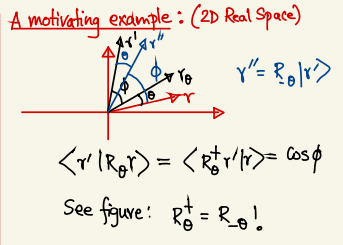
\includegraphics[width = 0.4 \textwidth]{Lecture12/2.png}
\subsection{Adjoint of the derivative operator}


The defining equation: $\left\langle o^{+} u \mid v\right\rangle=\langle u \mid 0 v\rangle$
Now consider two functions $ f(x), g(x)$


$$
\begin{aligned}
\int_{-\infty}^{\infty} d x\left(0^{+} f(x)\right)^{*} g(x) &=\int_{-\infty}^{\infty} d x f^{*}(x) \frac{d}{d x} g(x) \quad \text { Let } d g=d v \Rightarrow v=g \\
&=\left.f^{*} g\right|_{-\infty} ^{\infty}-\int_{-\infty}^{\infty} d x \frac{d f^{*}}{d x} g(x) \Rightarrow d f^{*}=d u \\
&=\int_{-\infty}^{\infty} d x\left(-\frac{d}{d x} f^{*} g(x)\right.
\end{aligned}
$$

\begin{itemize}
    \item Problem: $O=x \frac{d}{d x}$ find the adjoint: $O^+$
    \item $p \cong-i \hbar \frac{d}{d x}$; what is $p^{+?}$
\end{itemize}

\section{Hermitian Operators}

Note expectation values are given by $\braket{\hat{O}}_V = \braket{V|\hat{O}|V} \equiv \braket{V|\hat{O} V}$

Let us require such quantities to be real, for all $V$:

$$\braket{V|\hat{O}|V} \underbrace{=}_{\text{to be real}} \braket{V|\hat{O}|V}^* \underbrace{=}_{\text{definition of adjoint}} \braket{\hat{O}^+ V | V}^* \underbrace{=}_{\text{inner product property}}$$

$$\Rightarrow O = O^+$$

Such operators are called Hermitian. \textbf{ALL}
 observables in quantum mechanics are necessarily Hermitian. 
 
Question: If the variance of an observable is identically $O$ in a particle state for an operator $\hat{Q}$, prove that the state under consideration is an eigenstate of $\hat{a}$ with eigenvalue $\langle\hat{Q}\rangle$.

$$
\begin{aligned}
\left\langle\psi\left|\hat{Q}^{2}-\langle\hat{Q}\rangle^{2}\right| \psi\right\rangle=0 \Rightarrow &\langle\psi|(\hat{Q}-\langle\hat{Q}\rangle)(\hat{Q}-\langle\hat{Q}\rangle)| \psi\rangle=0 \\
\Rightarrow &\left\langle(\hat{Q}-\langle\hat{Q}\rangle)^{+} \psi|(\hat{Q}-\langle\hat{Q}))| \psi\right\rangle=0 \\
\Rightarrow &\langle(\hat{Q}-\langle\hat{Q}\rangle) \psi|(\hat{Q}-\langle\hat{Q}\rangle)| \psi\rangle=0 \text { ( Hermitian;  } \hat{Q}^+ = \hat{Q} ) \\
& \Rightarrow(\hat{Q}-\langle\hat{Q}\rangle)|\psi\rangle=0 \\
& \Rightarrow \hat{Q}|\psi\rangle=\langle\hat{Q}\rangle|\psi\rangle
\end{aligned}
$$

\subsubsection*{Geometric Interpretation}

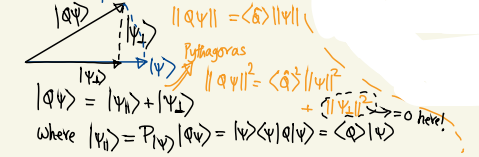
\includegraphics[width = 0.4 \textwidth]{Lecture12/3.png}

Question: Prove that the eigenvectors of any Hermitian operator (ignore degeneracy for now) will form an ONB for the space of vectors the operator acts on!
Consider eigenstates of $\hat{O}$ labelled by $\left\{\left|a_{i}\right\rangle\right\}_{i=1}^{N}$
$$
\left\langle a_{i}|\hat{O}| a_{j}\right\rangle=\left\langle a_{i}|\hat{0}+| a_{j}\right\rangle \Rightarrow a_{j}\left\langle a_{i} \mid a_{j}\right\rangle=a_{i}^{*}\left\langle a_{i} \mid a_{j}\right\rangle
$$


CaseI : $i=j \Rightarrow a_{i}=a_{i}^{*} \forall i \Rightarrow a_{i} \in \mathbb{R}$ for alli
$\left.\begin{array}{l}a_{j}\left\langle a_{i} \mid a_{j}\right\rangle=a_{i}\left\langle a_{i} \mid a_{j}\right\rangle \\ \text { case 2: } i \neq j \Rightarrow\left\langle a_{i} \mid a_{j}\right\rangle=0\end{array}\right\}$ Thus they form an ONB! One can fix the normalization for individual eigen vectors. 


This is a fundamental fact for QM
nomalization
\textbf{Any vector (later "quantum states") can be uniquely expanded in the eigen basis of ANY observable (later "Hermitian operator").}

\subsection{Uncountable / Continuous basis}

\begin{itemize}
    \item Bra and Ket vectors for definite position and momentum states of a 1D particle/system.
    \item Start with position: $x \leftarrow$ a Continuous variable.
    
    Basis states: $|x\rangle, \forall x \in \mathbb{R}$
    
    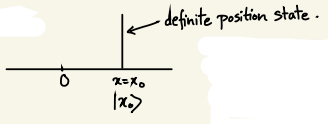
\includegraphics[width = 0.4 \textwidth]{Lecture12/4.png}
    
    Aside: Note that even in 3d, $\ket{\vec{r_1}  + \vec{r_2}} \neq \ket{\vec{r_1}} + \ket{\vec{r_2}}$
    
    \item The label inside the Ket is Not a vector.
    
    \hfill
    
\item  Inner pdt: $\langle x \mid y\rangle=\delta(x-y)$
$\langle x \mid x\rangle=\delta(0) \rightarrow \infty$
$\longrightarrow$ non-normalisable states. BUT, as in the free particle, they can be used to Construct normalisable physical states via (Continuous) superposition!
\item Completeness: $1=\int_{-\infty}^{\infty} d x|x\rangle\langle x|$
 $\int_{-\infty}^{\infty} d x \delta(x-y)|x\rangle=|y\rangle$
 
 \item Sanity check: $|y\rangle=\int_{-\infty}^{\infty} d x|x\rangle\langle x \mid y\rangle=\int_{-\infty}^{\infty} d x \delta{x-y} \ket{x} = \ket{y}$
 
 \item The position operator: $\underbrace{\hat{x}}_{\text{operator}}|x\rangle= \underbrace{x}_{\text{number}} \underbrace{|x\rangle}_{\text{eigenstates}}$
 
 
Check: $x^{+}=x:\left\langle x_{1}\left|\hat{x}^{+}\right| x_{2}\right\rangle=\left\langle x_{2}|x| x_{1}\right\rangle^{*}=x_{1} \delta\left(x_{2}-x_{1}\right)=x_{2} \delta\left(x_{1}-x_{2}\right)=\left\langle x_{1}|\hat{x}| x_{2}\right\rangle$

\item Also note: $\langle x| \hat{x}=x\langle x|$


\item Similar things for the momentum basis states: $|p\rangle ; \forall p \in \mathbb{R}$ and operator $\hat{p}$.

$$\left\langle p^{\prime} \mid p\right\rangle=\delta\left(p-p^{\prime}\right) ; 1=\int d p|p\rangle\langle p|; \hat{p}| p\rangle=p|p\rangle ;\langle p| \hat{p}=p\langle p| ; \hat{p}^{t}=\hat{p}$$

\end{itemize}


\subsection*{But all this math for what? Where is the quantum state / wavefunction?}

\begin{itemize}
    \item The fundamental postulate of quantum mechanics: The state of a quantum system is described by the state vector $\ket{\Psi(t)}$ which lives in a complex vector space (Hilbert space to be rigorous). So, $\ket{\Psi(t)} \in \mathbb{H}$
    
    \item What you have known so far as the (position-state) wavefunction is a mere projection of this state vector in the position basis. 
    
    $$\Psi(x,t) \equiv \braket{x|S(t)} \in \CC$$
    
    Note that $\psi(x) = \braket{x|\Psi} = \int dx' \braket{x|x'} \braket{x'|\Psi} = \int dx' \delta(x-x') \psi(x')$
    
    Similarly \footnote{You may recognize this as the Fourier transform} $\Tilde{\Psi} (p,t) \equiv \braket{p|\psi(t)}$
    
    $$\psi(x) \equiv \braket{x|\psi} = \int dp \braket{x|p} \braket{p|\psi} = \int dp \braket{x|p} \Tilde{\Psi} (p)$$
    
    This is the Fourier transform in disguise!
    
    Note that $\braket{x|p}$ will turn out to be equal to $\frac{e^{ipx\hbar}}{\sqrt{2 \pi \hbar}}$
\end{itemize}



\end{document}